\documentclass[12pt]{article}
\usepackage{fullpage} 
\usepackage{microtype}      % microtypography
\usepackage{array}
\usepackage{amsmath,amssymb,amsfonts}
\usepackage{amsthm}
\usepackage{graphicx}

%% Header
\usepackage{fancyhdr}
\fancyhf{}
\fancyhead[C]{CS 136 - 2022s - Checkpoint1 Submission}
\fancyfoot[C]{\thepage} % page number
\renewcommand\headrulewidth{0pt}
\pagestyle{fancy}

\usepackage[headsep=0.5cm,headheight=2cm]{geometry}

%% Hyperlinks always blue, no weird boxes
\usepackage[hyphens]{url}
\usepackage[colorlinks=true,allcolors=black,pdfborder={0 0 0}]{hyperref}

%%% Doc layout
\usepackage{parskip}
\usepackage{times}

%%% Write out problem statements in blue, solutions in black
\usepackage{color}
\newcommand{\officialdirections}[1]{{\color{blue} #1}}

%%% Avoid automatic section numbers (we'll provide our own)
\setcounter{secnumdepth}{0}

\begin{document}

\begin{center}
{\Large{\bf Student Names: Alexander Lobo and Nate Davis}}
\end{center}

{\Large{\bf Collaboration Statement:}}

Turning in this assignment indicates you have abided by the course Collaboration Policy:

\url{www.cs.tufts.edu/comp/136/2022s/index.html#collaboration-policy}

Total hours spent: 15

We consulted the following resources:
\begin{itemize}
\item Bishop Textbook
\item Course Videos
\item Various APIs/Stack Exchanges (e.g. sk-learn, TEX, imbalanced-learn, etc.)
\end{itemize}

\tableofcontents

\newpage

\section{General information about the data}

This dataset contains measures of distances within different shapes (conformations) of a set of 102 molecules. The study that this data comes from used human experts to judge the smell of each molecule and determine whether it is characterized as ``musk" or ``non-musk", which makes this a binary classification dataset.
\begin{itemize}
\item There are 6,598 conformations total (number of data points)
\item There are 166 features (not including the molecule and conformation names)
\item In the initial judgment, 39 of the molecules were assessed to be musks and 63 to be non-musks.
\end{itemize}

\section{Exploratory Data Analysis}

\subsection{Describing your analysis}

We followed the following data analysis steps to obtain a comprehensive understanding of our data:

\begin{enumerate}
\item \textbf{Visualized the marginal distribution of each feature}

\textit{Goal}: To understand the nature of the distributions of our features

\textit{Procedure}: Used a MinMax scaler on all values for a given feature and plotted histograms

\item \textbf{Visualized the marginal distribution of the output classes}

\textit{Goal}: To see whether the output classes were balanced or imbalanced

\textit{Procedure}: Plotted a histogram of the output values

\item \textbf{Analyzed the relationship between different features and between features and outcomes.}

\textit{Goal}: To see whether any sets of features exhibited similar distribution patterns and whether there was potentially some feature redundancy

\textit{Procedure}: Created a correlation matrix for the features and outcomes and plotted histograms of correlation values between different features and between features and outcomes.

\item \textbf{Visualized examples of joint distributions of pairs of the following features:}
\begin{enumerate}
\item Positively correlated features
\item Negatively correlated features
\item Uncorrelated features
\end{enumerate}

\textit{Goal}: To get a betters sense of how the joint distributions of each of these subgroups of feature pairs might look

\textit{Procedure}: Plotted joint plots of example pairs from each subgroups

\item \textbf{Conducted principal component analysis}

\textit{Goal}: To get a better sense of feature redundancy and see whether it would be feasible to cut down the feature set

\textit{Procedure}: Plotted the data with feature set condensed to 2 principle components; plotted \% variance retained by \# of principal components

\end{enumerate}

\subsection{Analyzing the results}

\subsubsection{General Trends}

The 166 features exhibit a wide variety of marginal distributions. Some look approximately normal, some multimodal, and others exponential. None, however, appears to be approximately uniform. Thus, each distribution displays at least one concentrated area of observations. As one might expect with the large number of features and variety of distributions, the feature set exhibits a range of correlations as well, with the distribution of feature-feature correlations looking approximately normal. The distribution of feature-outcome correlations, however, is much narrower, with no features showing high positive or negative correlation with musk classification. Given the large number of features, it is useful to note that via principal component analysis we can winnow the set down to about 20-30 variables while maintaining greater than 80\% of the original variance.

The distribution of output classes is quite imbalanced, with non-musk conformations greatly outnumbering musks. This could potentially present an issue when training a model as musk-classified training examples will be few and far between.

\subsubsection{Marginal Distribution of Features}

\begin{center}
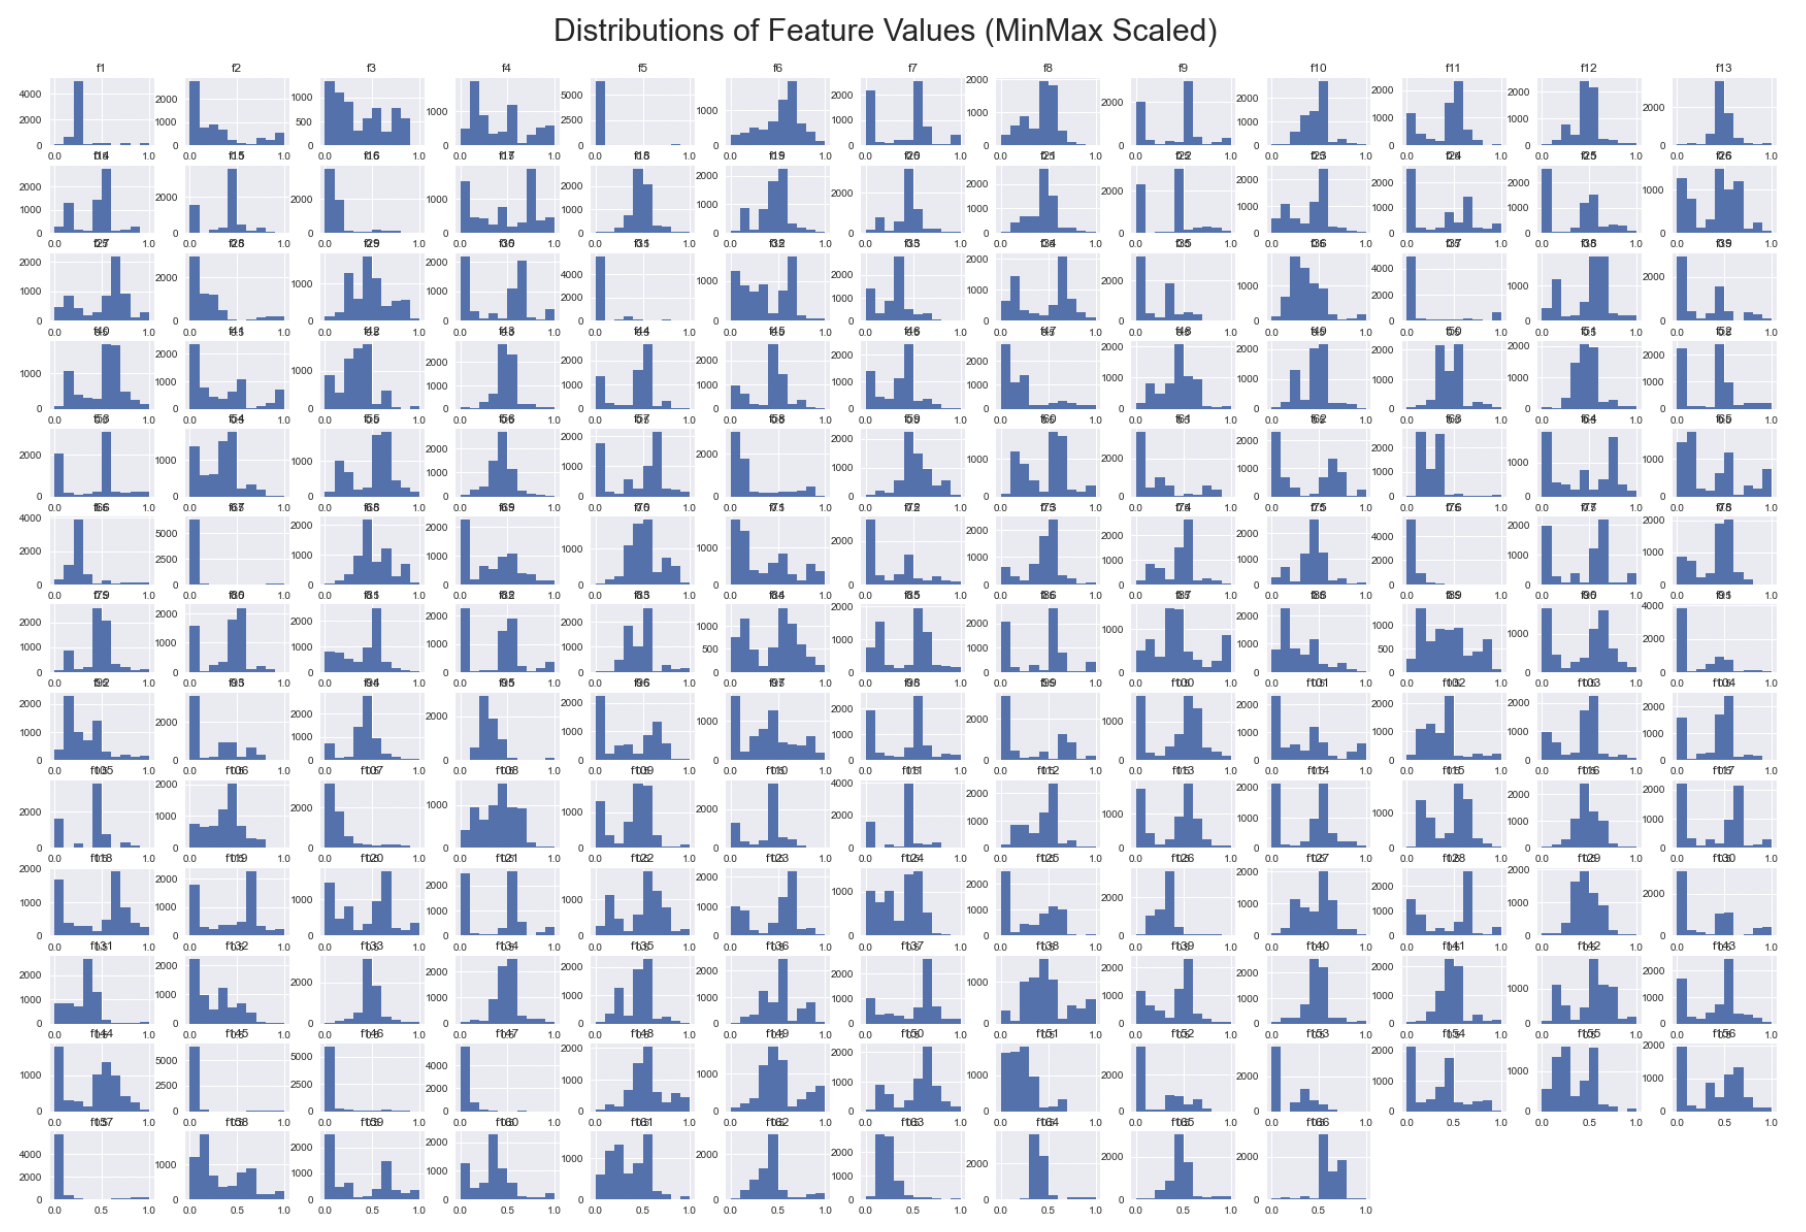
\includegraphics[scale=.35]{feature_distribs.jpg}
\end{center}

As we can see above, the features of this data set exhibit a wide variety of distributions, some vaguely normal, others multimodal or even exponential. None appear uniform, so each molecular axis has at least one area along which observations are clustered. Additionally, few if any concentrations of observations occur at the high end of these scaled ranges. This implies that there is a tendency for observations to fall at the lower end of these distances, which are typically negative. The original analysis of this data set says that the 0 points on these axes are arbitrary, so it's hard to glean much meaning from this, but interesting to note nonetheless.

If we look at a histogram compiling all of these scaled observations, we can see these general trends writ large, with the overall mix of distributions combining to make what looks like a normal distribution combined with an exponential distribution. Thus, the molecular distances appear to be drawn from a mixed model.

\begin{center}
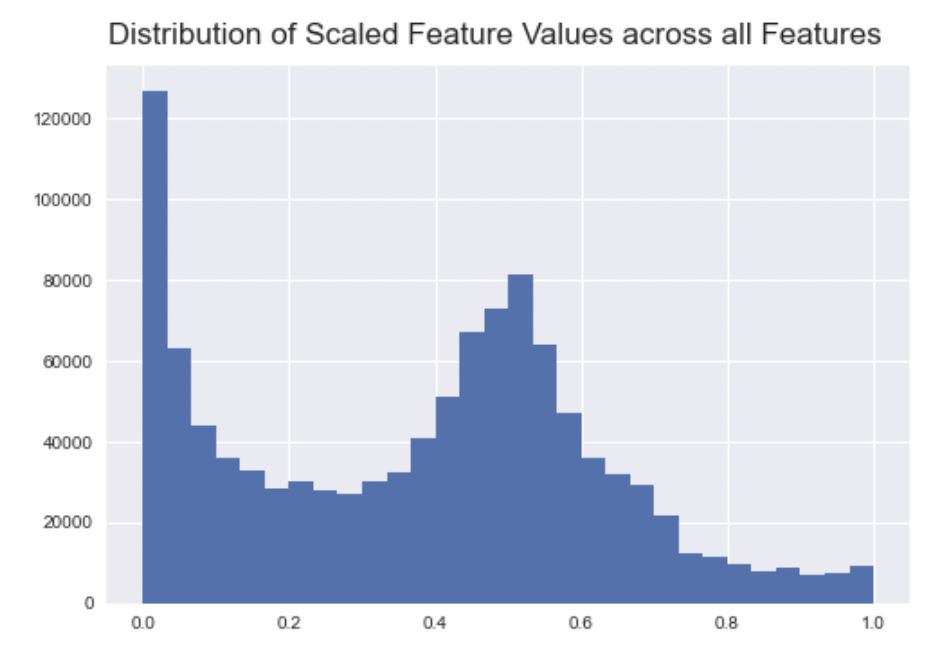
\includegraphics[scale=.35]{all_feature_distrib.jpg}
\end{center}

\subsubsection{Feature-Feature and Feature-Outcome Correlations}

\begin{center}
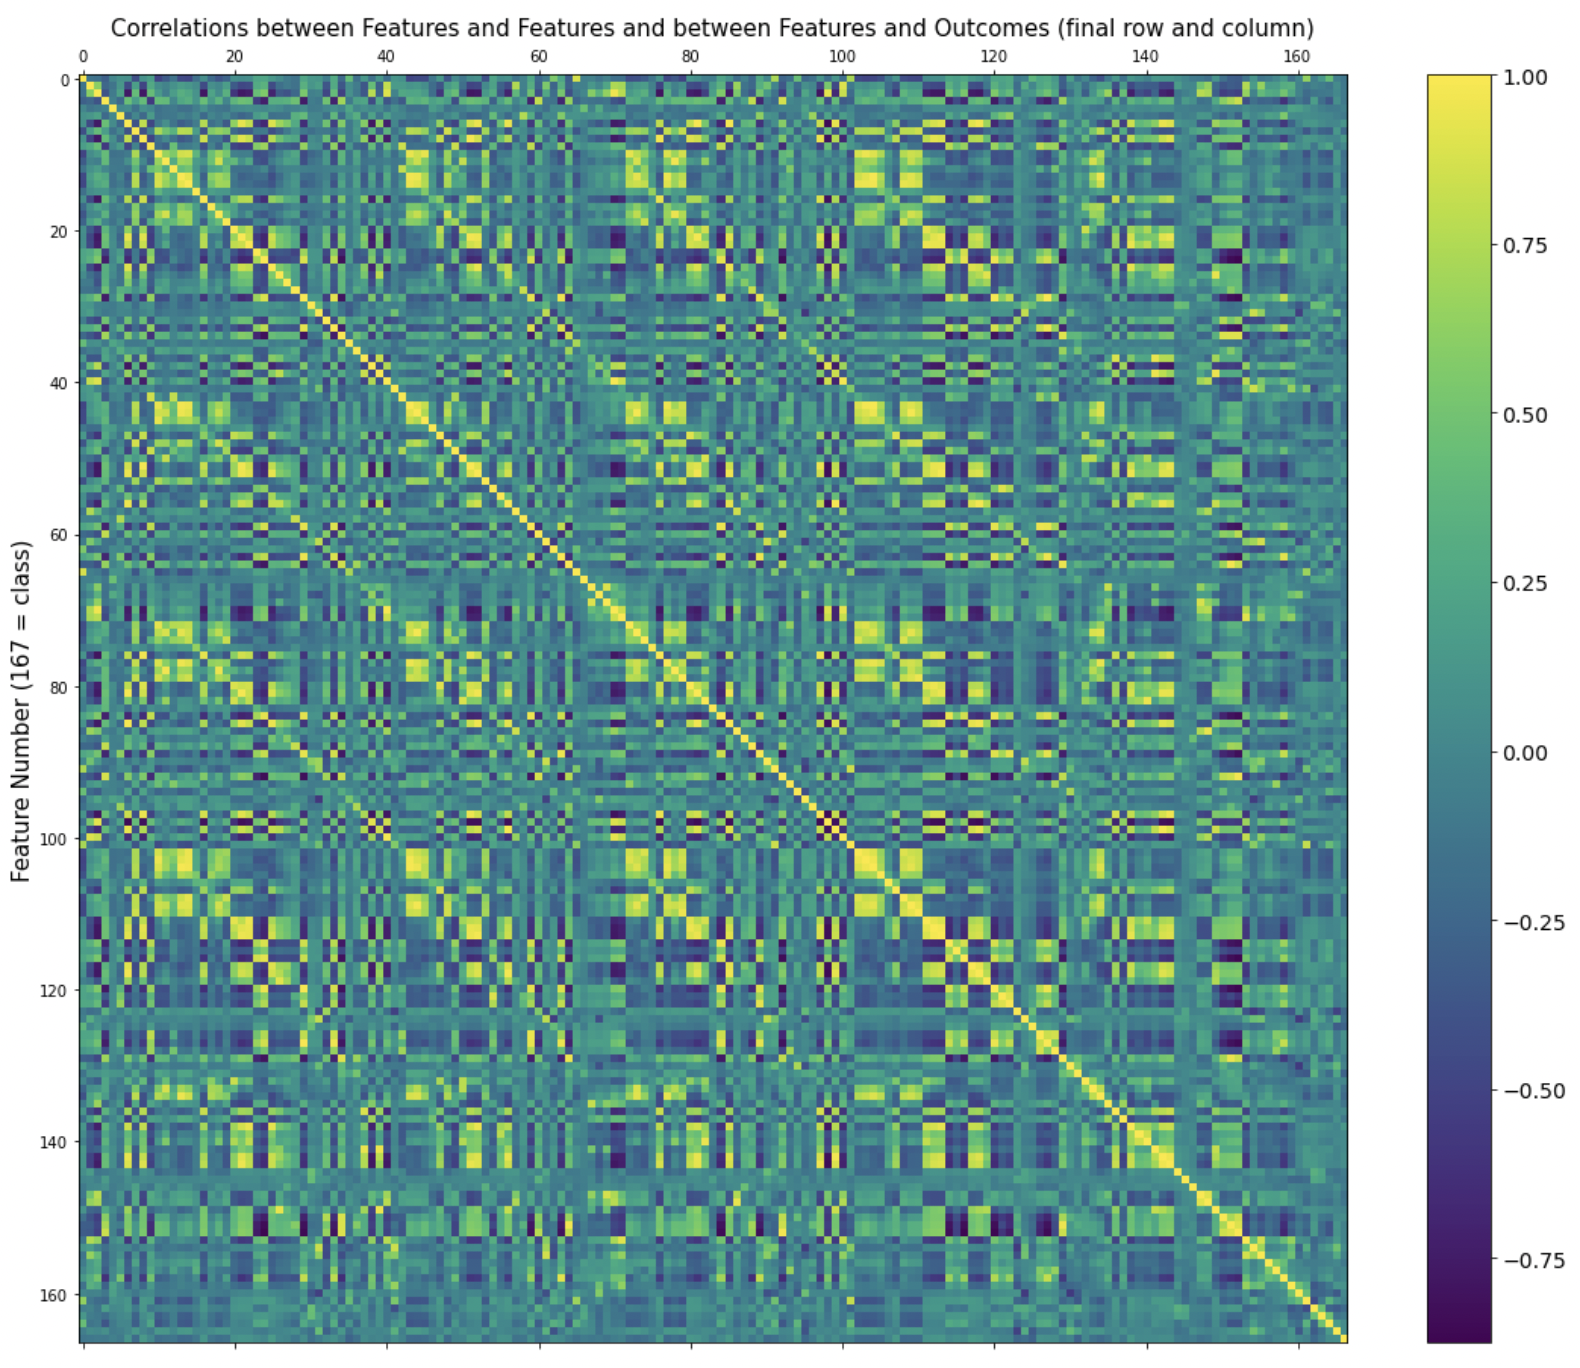
\includegraphics[scale=0.5]{correlation_matrix.jpg}
\end{center}

There are some interesting patterns in terms of feature-feature correlations in this data set. As is easily seen in the correlation matrix above, there are a handful of series of successively numbered features that exhibit high positive correlation with other series of successively numbered features. This results in the various diagonal yellow lines around the matrix (not including the main diagonal, of course). We can see that in the feature-feature correlations (all squares except for the last row and column) there are also a large number of highly negative correlations. On the whole, there is quite a range, so it makes sense when viewed in a histogram. The set of correlations appears to be approximately normally distributed.

\begin{center}
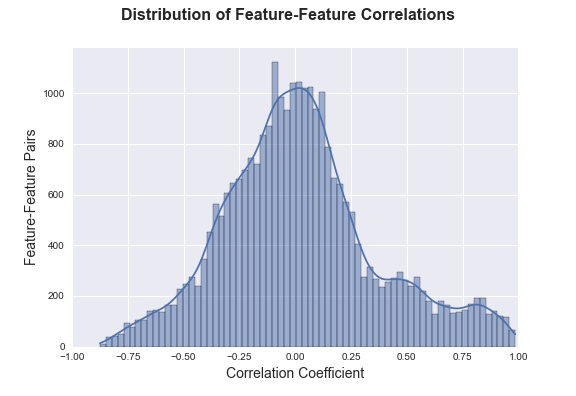
\includegraphics[scale=0.5]{figures/feature_feature_corr.jpg}
\end{center}

The final row and column of the correlation matrix, which contain feature-outcome correlations, while hard to make out, don't appear to have many very high or low values. This visual inspection is confirmed by looking at the distribution of these values. As you can see below, it is much narrower than that of the feature-feature correlations, meaning that no feature is in and of itself highly predictive of the outcome. Thus, the whole procedure of training a model using multiple of these features makes sense.

\begin{center}
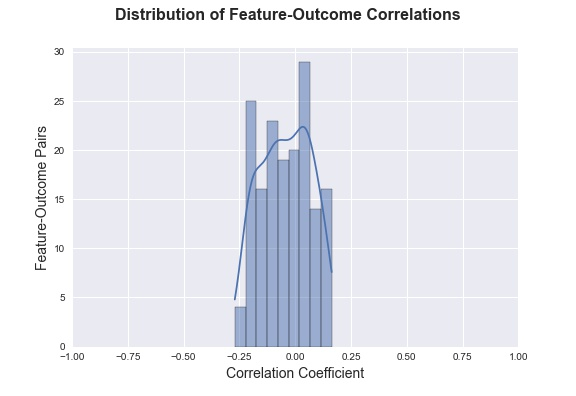
\includegraphics[scale=0.5]{figures/feature_outcome_corr.jpg}
\end{center}

\subsubsection{Joint Feature Distributions}

After exploring the correlations between features, we explored the joint distributions between a select few that have a highly positive correlation, a highly negative correlation, and no correlation. The marginal distributions of the selected features are shown below:

\begin{center}
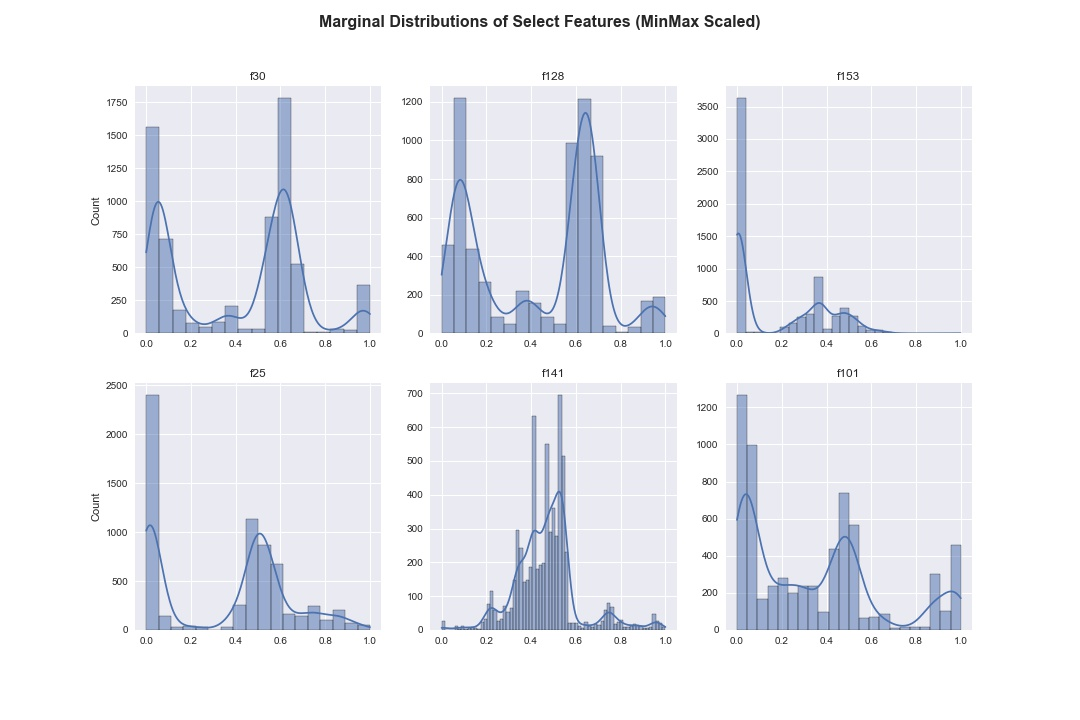
\includegraphics[scale=0.4]{figures/select_marginals.jpg}
\end{center}

The joint distributions are shown below:

\begin{figure}[!htb]
\minipage{0.32\textwidth}
  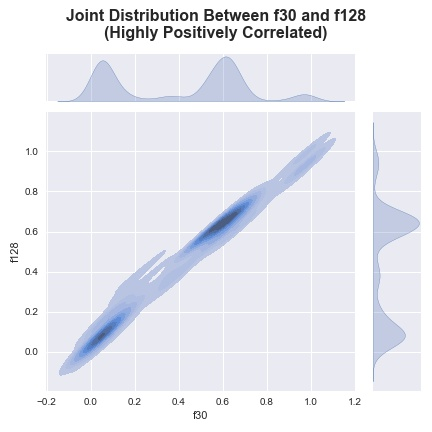
\includegraphics[width=\linewidth]{figures/joint_marginals_high_corr.jpg}
\endminipage\hfill
\minipage{0.32\textwidth}
  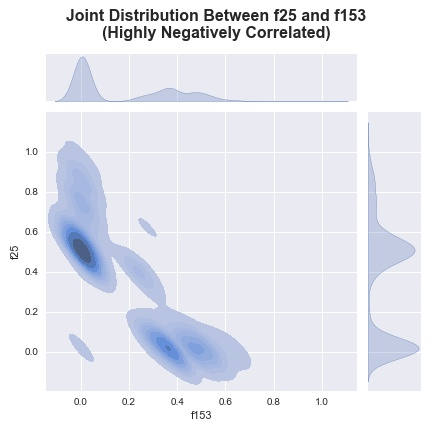
\includegraphics[width=\linewidth]{figures/joint_marginals_neg_corr.jpg}
\endminipage\hfill
\minipage{0.32\textwidth}%
  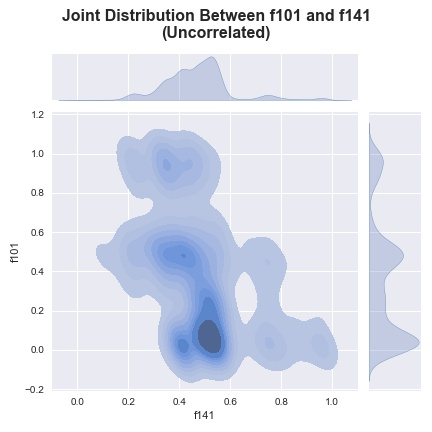
\includegraphics[width=\linewidth]{figures/joint_marginals_un_corr.jpg}
\endminipage
\end{figure}

We expect feature redundancy between features that are highly positively or negatively uncorrelated. Ultimately, our model should be built using features that are fairly uncorrelated, especially considering  the lack of feature-outcome correlations.

\subsubsection{Principal Component Analysis}

It might be helpful to reduce the number of features since there are many in our data set, which can unnecessarily increase the time it takes to train a model. By utilizing principal component analysis we can visualize the variance retained with each incremental increase in number of principal components. As we can see from the graph below, we can cut the number of features down to 14 principal components and still retain over 80\% of the original variance. To retain 90\%, we would need 26, and to get 99\%, we would need 74. Even at this high bar, we could significantly reduce our feature set by more than half. This ability to reduce the feature space makes sense in light of the number of features with very high (positive) and very low (negative) correlations.

\begin{center}
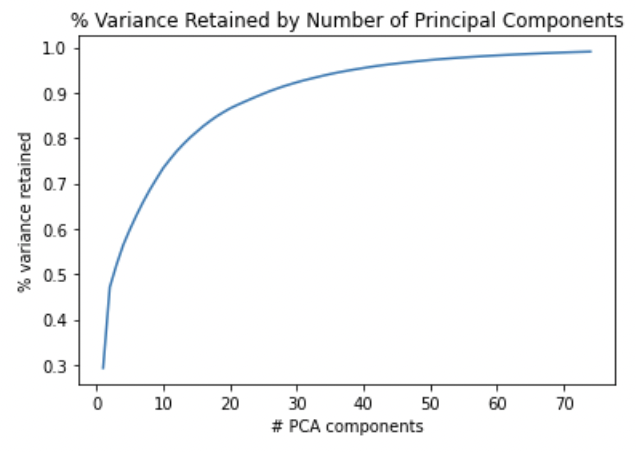
\includegraphics[scale=0.8]{pca_var_retained.jpg}
\end{center}

\subsubsection{Outcome Distribution}

The outcome distribution is highly imbalanced, with approximately 85\% of the conformations being classified as non-musks. This is even more imbalanced than the molecule outcome distribution, in which approximately 60\% of molecules were judged to be non-musks. This means that non-musk molecules have about 40\% more conformations on average than musk molecules.

\begin{center}
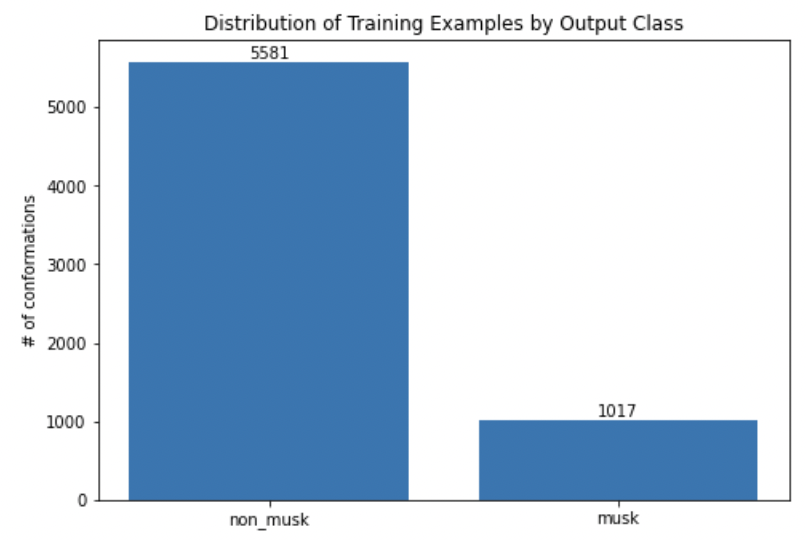
\includegraphics[scale=0.8]{outcome_distrib.jpg}
\end{center}

For training a logistic classifier, we may need to take this imbalance into account in order to train a model most efficiently. We could account for this aspect of the data either by weighing errors on musk conformations higher than those on non-musks during gradient descent or by using an ensemble model, in which each iteration of the classification model puts a higher weight on the loss associated with observations misclassified by models that came before. We could also consider an oversampling technique, such as SMOTE\footnote{\url{https://towardsdatascience.com/smote-fdce2f605729}}, to balance the output classes.

\newpage

\section{Model and Learning Method Properties}
  
\subsection{Model}

We will be using a logistic regression model with a Bernoulli likelihood for the outcome given a logistic sigmoid link function and a multivariate Gaussian prior on the weight vector for this data set. The likelihood for this model is the probability of seeing our training data given a certain weight vector. Equations for our likelihood and prior are given below.

Firstly, the posterior probability of class $\mathcal{C}_1$ is written as a logistic sigmoid in a linear function of the feature vector such that

\begin{equation}
	y_n = p(\mathcal{C}_1|\phi(x_n)) = \sigma(\textbf{w}^\top \phi(x_n))
\end{equation}

where $\sigma(\cdot)$ is the logistic sigmoid function and $p(\mathcal{C}_2|\phi(x_n)) = 1 - p(\mathcal{C}_1|\phi(x_n))$.

\subsubsection{Prior}

The prior is given by

\begin{equation}
    p(\textbf{w}|\alpha) = \mathcal{N}(\vec{0}, \alpha^{-1}I_{166})
\end{equation}

where $\alpha$ is the presumed precision of each weight component (each assumed to be 0).

\subsubsection{Likelihood}

The likelihood for a single outcome is given below.

\begin{equation}
    p(t_n|\textbf{w}) = \mathrm{Bern}(t_n | \sigma(\textbf{w}^\top \phi(x_n))
\end{equation}

Assuming that all outcomes are independently and identically distributed (i.i.d), we can then write the likelihood of all of the outcomes as the following:

\begin{align}
    p(\textbf{t}|\textbf{w}) &= \prod_{n=1}^N \mathrm{Bern}(t_n | \sigma(\textbf{w}^\top\phi(x_n)) \\
    	&= \prod_{n=1}^N y_n^{t_n}(1-y_n)^{1-t_n}
\end{align}

where $\textbf{t} = (t_1, \ldots, t_N)^\top$ and $t_n \in {0,1}$.

By taking the logarithm of the the likelihood, we can find a maximum likelihood solution for the weight vector by finding the weight vector that maximizes the log likelihood:

\begin{align}
    \hat{\textbf{w}}_{\mathrm{ML}} &= \arg\max_{\textbf{w} \in \mathbb{R}^M} \log p(\textbf{t}|\textbf{w}) \\
    &= \arg \max_{\textbf{w} \in \mathbb{R}^M} \sum_{n=1}^N \log p(t_n|\textbf{w})
\end{align}

This can be achieve by computing the gradient of the log likelihood and setting the equation equal to 0. Although, a closed form analytical solution does not exist, which is why we must depend on gradient descent to find an answer. However, maximizing the log likelihood is tantamount to non-probabilistic logistic regression. Hence, we turn to the posterior distribution.

\subsubsection{Posterior}

The log posterior distribution is given by the following formula:

\begin{equation}
    \log p(\textbf{w}|\textbf{t}) = \underbrace{\sum_{n=1}^N \log p(t_n|\textbf{w})}_{\mathrm{Likelihood}} + \underbrace{\log p(\textbf{w}|\alpha)}_{\mathrm{Prior}} - \underbrace{\log p(\textbf{t})}_{\mathrm{Evidence}}
\end{equation}

The analytical solution for the posterior is difficult to solve. Luckily, we are only interested in the maximum a posteriori (MAP) estimate for the weight vector, which does not require the evidence to compute since it is constant with respect to $\mathbf{w}$ and is given by

\begin{align}
    \hat{\textbf{w}}_{\mathrm{MAP}} &= \arg\max_{\textbf{w} \in \mathbb{R}^M} \log p(\textbf{w}|\textbf{t}) \\
    &= \arg\max_{\textbf{w} \in \mathbb{R}^M} \sum_{n=1}^N \log p(t_n|\textbf{w}) + \log p(\textbf{w}|\alpha)
\end{align}

As before with the ML estimate, a closed form solution does not exist with the MAP estimate, which is why we must depend on first order and second order gradient descent to find a solution, which are the methods we will explore in this project.

\subsection{Learning method (inference)}

The primary parameter we will be learning from the data is the weight vector $\textbf{w}$. As stated before, we will be finding a MAP estimate for $\textbf{w}$ by performing first and second order gradient descent on the log posterior. The only other parameter that could be learnt from the data is the hyperparameter $\alpha$, which is the prior assumed precision of the 0 mean weight vector. In a probabilistic sense, learning $\alpha$ would require maximizing the evidence, which would require an approximation of the posterior distribution to compute an approximation of the evidence. However, we will not be exploring this method and instead will be using a grid search with k-fold cross validation to find the $\alpha$ that maximizes the log posterior.

\section{Performance Hypotheses}

The purpose of this study is to explore how our model performs when upgrading our learning method from a first order to a second order gradient descent algorithm to solve the weight vector MAP estimate for logistic regression. We propose the following hypotheses for how we expect our model to perform:

\begin{enumerate}
\item \textbf{We hypothesize that the time needed to compute the weight vectors will decrease after upgrading from a first order to second order gradient descent.}

We intend to measure the the time it takes to train the model with each method using the \texttt{time} library in Python to take the difference between start and end times. By doing so, we will be able to compare the computational time between the two methods to see which one is faster.

\item \textbf{We hypothesize that incorporating a higher weight penalty on false negative predictions (musk conformations labeled non-musk) will help improve the positive predictive value (precision) of the model.}

As discovered during our analysis, the output class is quite imbalanced, so we expect that incorporating a penalty will help mitigate any loss in precision. We will generate a confusion matrix to measure any changes in model performance.

\item \textbf{We hypothesize that projection the data onto 10-20 principal components will significantly reduce the training time of the model without much detriment to the prediction accuracy.}

Our preliminary PCA analysis showed a high retention of data set variance with 10-20 principal components. We will once again measure model performance with a confusion matrix and computational time with the \texttt{time} library to test our hypothesis.

\end{enumerate}

\end{document}